\documentclass[11pt]{article}
\usepackage[a4paper,landscape,margin=0.5cm]{geometry}
\usepackage{tikz}
\usepackage{graphicx}
\usepackage{amsmath}
\usepackage[T1]{fontenc}
\usepackage{helvet}
\renewcommand{\familydefault}{\sfdefault}
\usepackage{xcolor}
\usepackage{array}
\usetikzlibrary{calc}
\pagestyle{empty}

\begin{document}

% Header
\noindent
{\Huge\bfseries 10 Hygiea \& Gaia DR3 1234567890123456}\\[0.2cm]
{\huge 2026 gen 09 \quad 1$^{\mathsf{h}}$8$^{\mathsf{m}}$35.8$^{\mathsf{s}}$ U.T.}

\vspace{0.5cm}

\noindent
\begin{minipage}[t]{0.48\textwidth}
  \textbf{Planet:} \hfill a = 3.14, e = 0.117\\[0.1cm]
  V. mag. = 10.20 \quad Diam. = 407.1 km = 0.20"\\
  $\mu$ = 25.8"/h \quad $\pi$ = 2.1" \quad Ref. = JPL\#659
  
  \vspace{0.2cm}
  
  $\Delta$m = 7.45 \quad\quad Max. dur. = 22.2s
  
  \vspace{0.4cm}
  
  \textbf{Star:} \hfill Source cat. Gaia DR3\\[0.1cm]
  $\alpha$ = 8$^{\mathsf{h}}$13$^{\mathsf{m}}$49.6$^{\mathsf{s}}$ \quad\quad $\delta$ = +23°27'24.1"\\
  Vmag = 10.2 \quad\quad Bmag = 10.5
  
  \vspace{0.2cm}
  
  Sun: 161° \quad\quad Moon: 65°, 3\%
\end{minipage}
\hfill
\begin{minipage}[t]{0.48\textwidth}
  \textbf{Observability from Italy:}\\[0.2cm]
  \begin{tabular}{lccc}
    \textbf{Location} & \textbf{Alt} & \textbf{Az} & \textbf{Status} \\
    \hline
    Roma & 52° & 179° & Excellent \\
    Napoli & 49° & 175° & Excellent \\
    Firenze & 56° & 182° & Excellent \\
  \end{tabular}
  
  \vspace{0.3cm}
  
  Path uncertainty: $\pm$18 km\\
  Time uncertainty: $\pm$3.2 s\\
  Priority: {\Large\bfseries $\star\star\star$} (11/11)
\end{minipage}

\vspace{0.8cm}

% Main content with two panels
\noindent
\begin{minipage}[t]{0.48\textwidth}
  \centering
  % Star field panel
  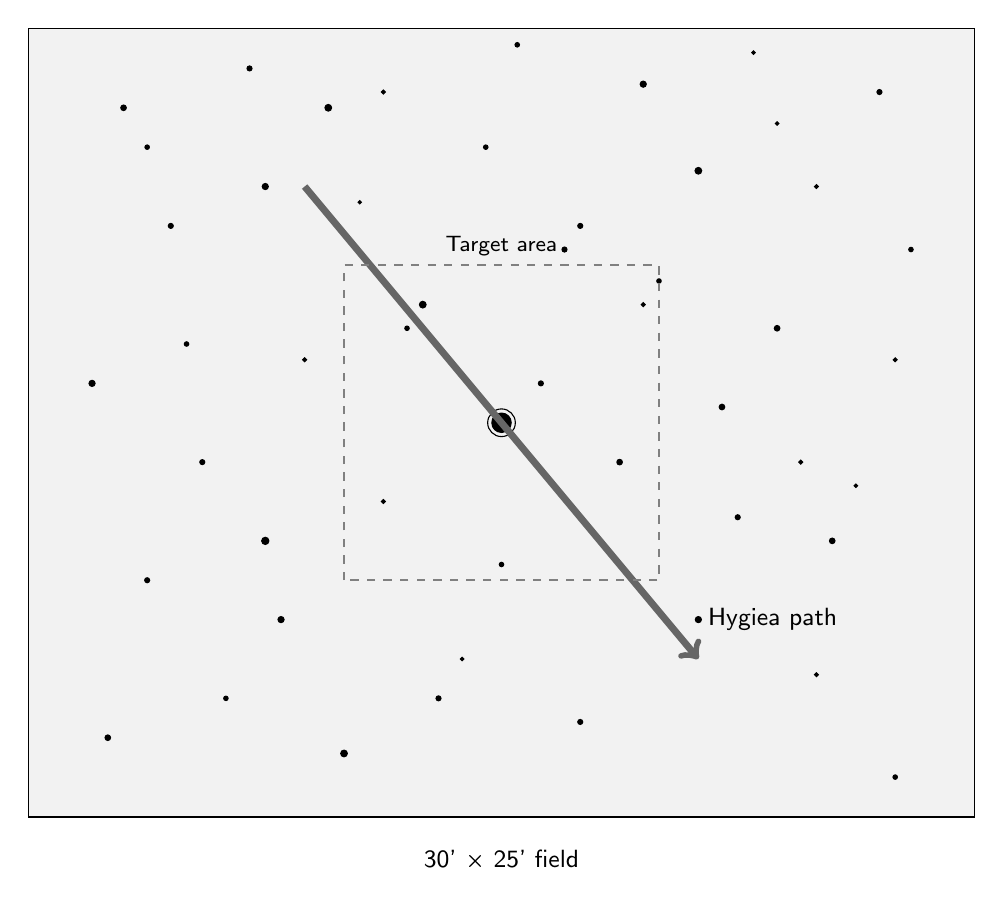
\begin{tikzpicture}
    % Border
    \draw[line width=1pt] (0,0) rectangle (12,10);
    
    % Background
    \fill[black!5] (0,0) rectangle (12,10);
    
    % Random stars (realistic field)
    \foreach \x/\y/\s in {
      1/1/1, 2.5/1.5/0.8, 4/0.8/1.2, 5.5/2/0.6, 7/1.2/0.9,
      8.5/2.5/1.1, 10/1.8/0.7, 11/0.5/0.8, 1.5/3/0.9, 3/3.5/1.3,
      4.5/4/0.7, 6/3.2/0.8, 7.5/4.5/1, 9/3.8/0.9, 10.5/4.2/0.6,
      0.8/5.5/1.1, 2/6/0.8, 3.5/5.8/0.7, 5/6.5/1.2, 6.5/5.5/0.9,
      8/6.8/0.8, 9.5/6.2/1, 11/5.8/0.7, 1.8/7.5/0.9, 3/8/1.1,
      4.2/7.8/0.6, 5.8/8.5/0.8, 7/7.5/0.9, 8.5/8.2/1.2, 10/8/0.7,
      11.2/7.2/0.8, 1.2/9/1, 2.8/9.5/0.9, 4.5/9.2/0.7, 6.2/9.8/0.8,
      7.8/9.3/1.1, 9.2/9.7/0.6, 10.8/9.2/0.9, 2.2/4.5/0.9, 8.8/5.2/1,
      4.8/6.2/0.8, 9.8/4.5/0.7, 3.2/2.5/1.1, 6.8/7.2/0.9, 1.5/8.5/0.8,
      10.2/3.5/1, 5.2/1.5/0.9, 7.8/6.5/0.7, 3.8/9/1.2, 9.5/8.8/0.6
    } {
      \filldraw[black] (\x,\y) circle (\s pt);
    }
    
    % Target star (larger, prominent)
    \filldraw[black] (6,5) circle (3.5pt);
    \draw[black] (6,5) circle (5pt);
    
    % Asteroid path with arrow
    \draw[->,line width=2.5pt,black!60] (3.5,8) -- (8.5,2);
    \node[right,font=\small] at (8.5,2.5) {Hygiea path};
    
    % Dotted box around target (finder field)
    \draw[dashed,black!50,line width=0.8pt] (4,3) rectangle (8,7);
    \node[above,font=\footnotesize] at (6,7) {Target area};
    
    % Coordinate labels
    \node[below,font=\small] at (6,-0.3) {30' × 25' field};
  \end{tikzpicture}
\end{minipage}
\hfill
\begin{minipage}[t]{0.48\textwidth}
  \centering
  % Earth map panel
  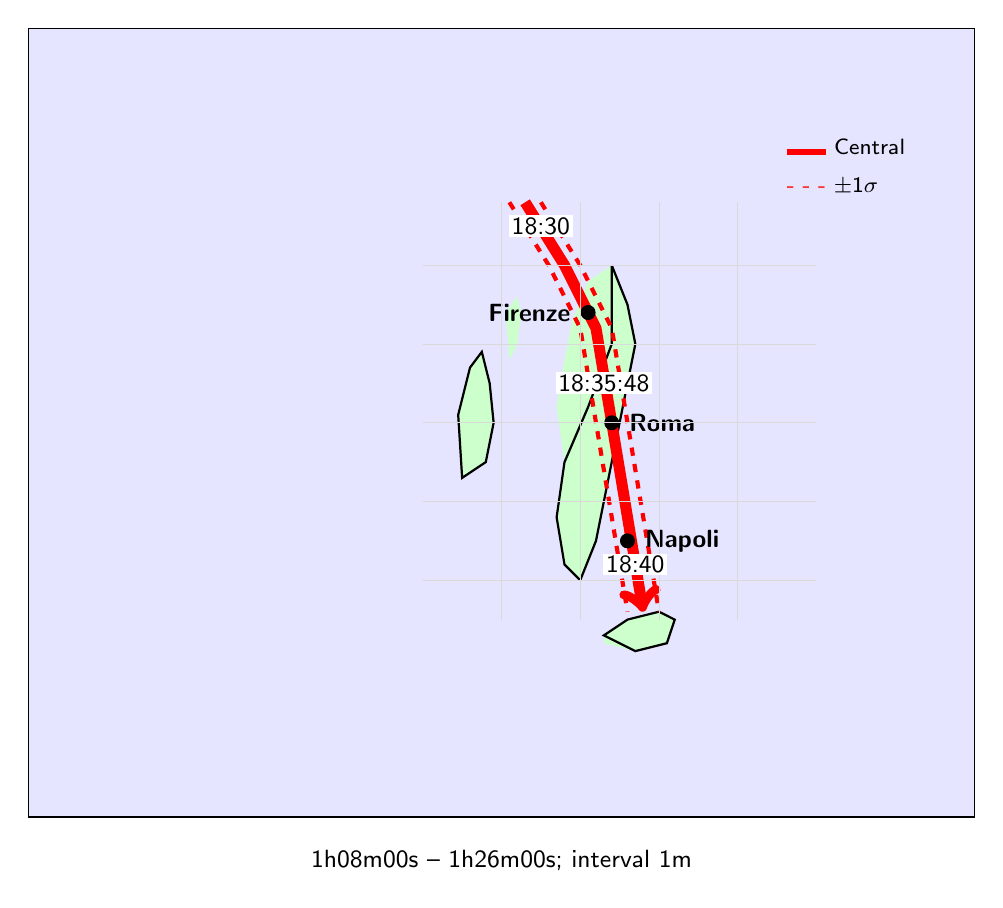
\begin{tikzpicture}
    % Border
    \draw[line width=1pt] (0,0) rectangle (12,10);
    
    % Ocean background
    \fill[blue!10] (0,0) rectangle (12,10);
    
    % Land (Italy and surroundings)
    % Mainland Italy
    \fill[green!20] (7,3) -- (7.2,3.5) -- (7.3,4) -- (7.4,4.5) -- (7.5,5) 
                       -- (7.6,5.5) -- (7.7,6) -- (7.6,6.5) -- (7.4,7)
                       -- (7.1,6.8) -- (6.9,6.3) -- (6.8,5.8) -- (6.7,5.2)
                       -- (6.8,4.5) -- (6.7,3.8) -- (6.8,3.2) -- cycle;
    
    % Sicily
    \fill[green!20] (7.3,2.3) -- (7.6,2.5) -- (8,2.6) -- (8.2,2.5) -- (8.1,2.2) -- (7.7,2.1) -- (7.3,2.2) -- cycle;
    
    % Sardinia
    \fill[green!20] (5.5,4.3) -- (5.8,4.5) -- (5.9,5) -- (5.85,5.5) -- (5.75,5.9) -- (5.6,5.7) -- (5.45,5.1) -- (5.5,4.3) -- cycle;
    
    % Corsica
    \fill[green!20] (6.1,5.8) -- (6.2,6) -- (6.25,6.4) -- (6.2,6.6) -- (6.05,6.4) -- (6.1,5.8) -- cycle;
    
    % Coastlines (darker)
    \draw[thick,black] (7,3) -- (7.2,3.5) -- (7.3,4) -- (7.4,4.5) -- (7.5,5) 
                       -- (7.6,5.5) -- (7.7,6) -- (7.6,6.5) -- (7.4,7);
    \draw[thick,black] (7,3) -- (6.8,3.2) -- (6.7,3.8) -- (6.8,4.5) -- (7.1,5.2) -- (7.4,6) -- (7.4,7);
    \draw[thick,black] (7.3,2.3) -- (7.6,2.5) -- (8,2.6) -- (8.2,2.5) -- (8.1,2.2) -- (7.7,2.1) -- cycle;
    \draw[thick,black] (5.5,4.3) -- (5.8,4.5) -- (5.9,5) -- (5.85,5.5) -- (5.75,5.9) -- (5.6,5.7) -- (5.45,5.1) -- cycle;
    
    % Central path (thick red line with arrow)
    \draw[->,line width=4pt,red] (6.3,7.8) -- (6.8,7) -- (7.2,6.2) -- (7.4,5) -- (7.6,3.8) -- (7.8,2.6);
    
    % Uncertainty limits (dashed red)
    \draw[dashed,red,line width=1.5pt] (6.5,7.8) -- (7,7) -- (7.4,6.2) -- (7.6,5) -- (7.8,3.8) -- (8,2.6);
    \draw[dashed,red,line width=1.5pt] (6.1,7.8) -- (6.6,7) -- (7,6.2) -- (7.2,5) -- (7.4,3.8) -- (7.6,2.6);
    
    % Cities (with dots and labels)
    \filldraw[black] (7.4,5) circle (2.5pt);
    \node[right,font=\small\bfseries] at (7.5,5) {Roma};
    
    \filldraw[black] (7.6,3.5) circle (2.5pt);
    \node[right,font=\small\bfseries] at (7.7,3.5) {Napoli};
    
    \filldraw[black] (7.1,6.4) circle (2.5pt);
    \node[left,font=\small\bfseries] at (7,6.4) {Firenze};
    
    % Coordinate grid (subtle)
    \foreach \lat in {3,4,5,6,7} {
      \draw[gray!30,very thin] (5,\lat) -- (10,\lat);
    }
    \foreach \lon in {6,7,8,9} {
      \draw[gray!30,very thin] (\lon,2.5) -- (\lon,7.8);
    }
    
    % Time markers along path
    \node[font=\small,fill=white,inner sep=1pt] at (6.5,7.5) {18:30};
    \node[font=\small,fill=white,inner sep=1pt] at (7.3,5.5) {18:35:48};
    \node[font=\small,fill=white,inner sep=1pt] at (7.7,3.2) {18:40};
    
    % Labels
    \node[below,font=\small] at (6,-0.3) {1h08m00s -- 1h26m00s; interval 1m};
    
    % Legend
    \node[anchor=west,font=\footnotesize] at (9.5,8.5) {\textcolor{red}{\rule{0.5cm}{2pt}} Central};
    \node[anchor=west,font=\footnotesize] at (9.5,8) {\textcolor{red}{- - -} $\pm$1$\sigma$};
  \end{tikzpicture}
\end{minipage}

\vspace{0.4cm}

\noindent
{\footnotesize\textbf{Equipment recommendations:} GPS timing device essential. Video recording at 25+ fps recommended. Telescope aperture >20cm for mag 10.2 star.}

\vspace{0.2cm}

\noindent
{\footnotesize Generated by ITALOccultCalc v1.0 -- Predictions: JPL DE441, Gaia DR3 -- For IOTA coordination}

\end{document}
